\section{Effets :}
\textbf{NB:} Tous les effets nécessitant un histogramme utilise celui de la "\emph{valeur}", soit le maximum entre les trois canaux de l'espace de couleur Rouge Vert Bleu.

\subsection{Luminosité (Brightness) :}
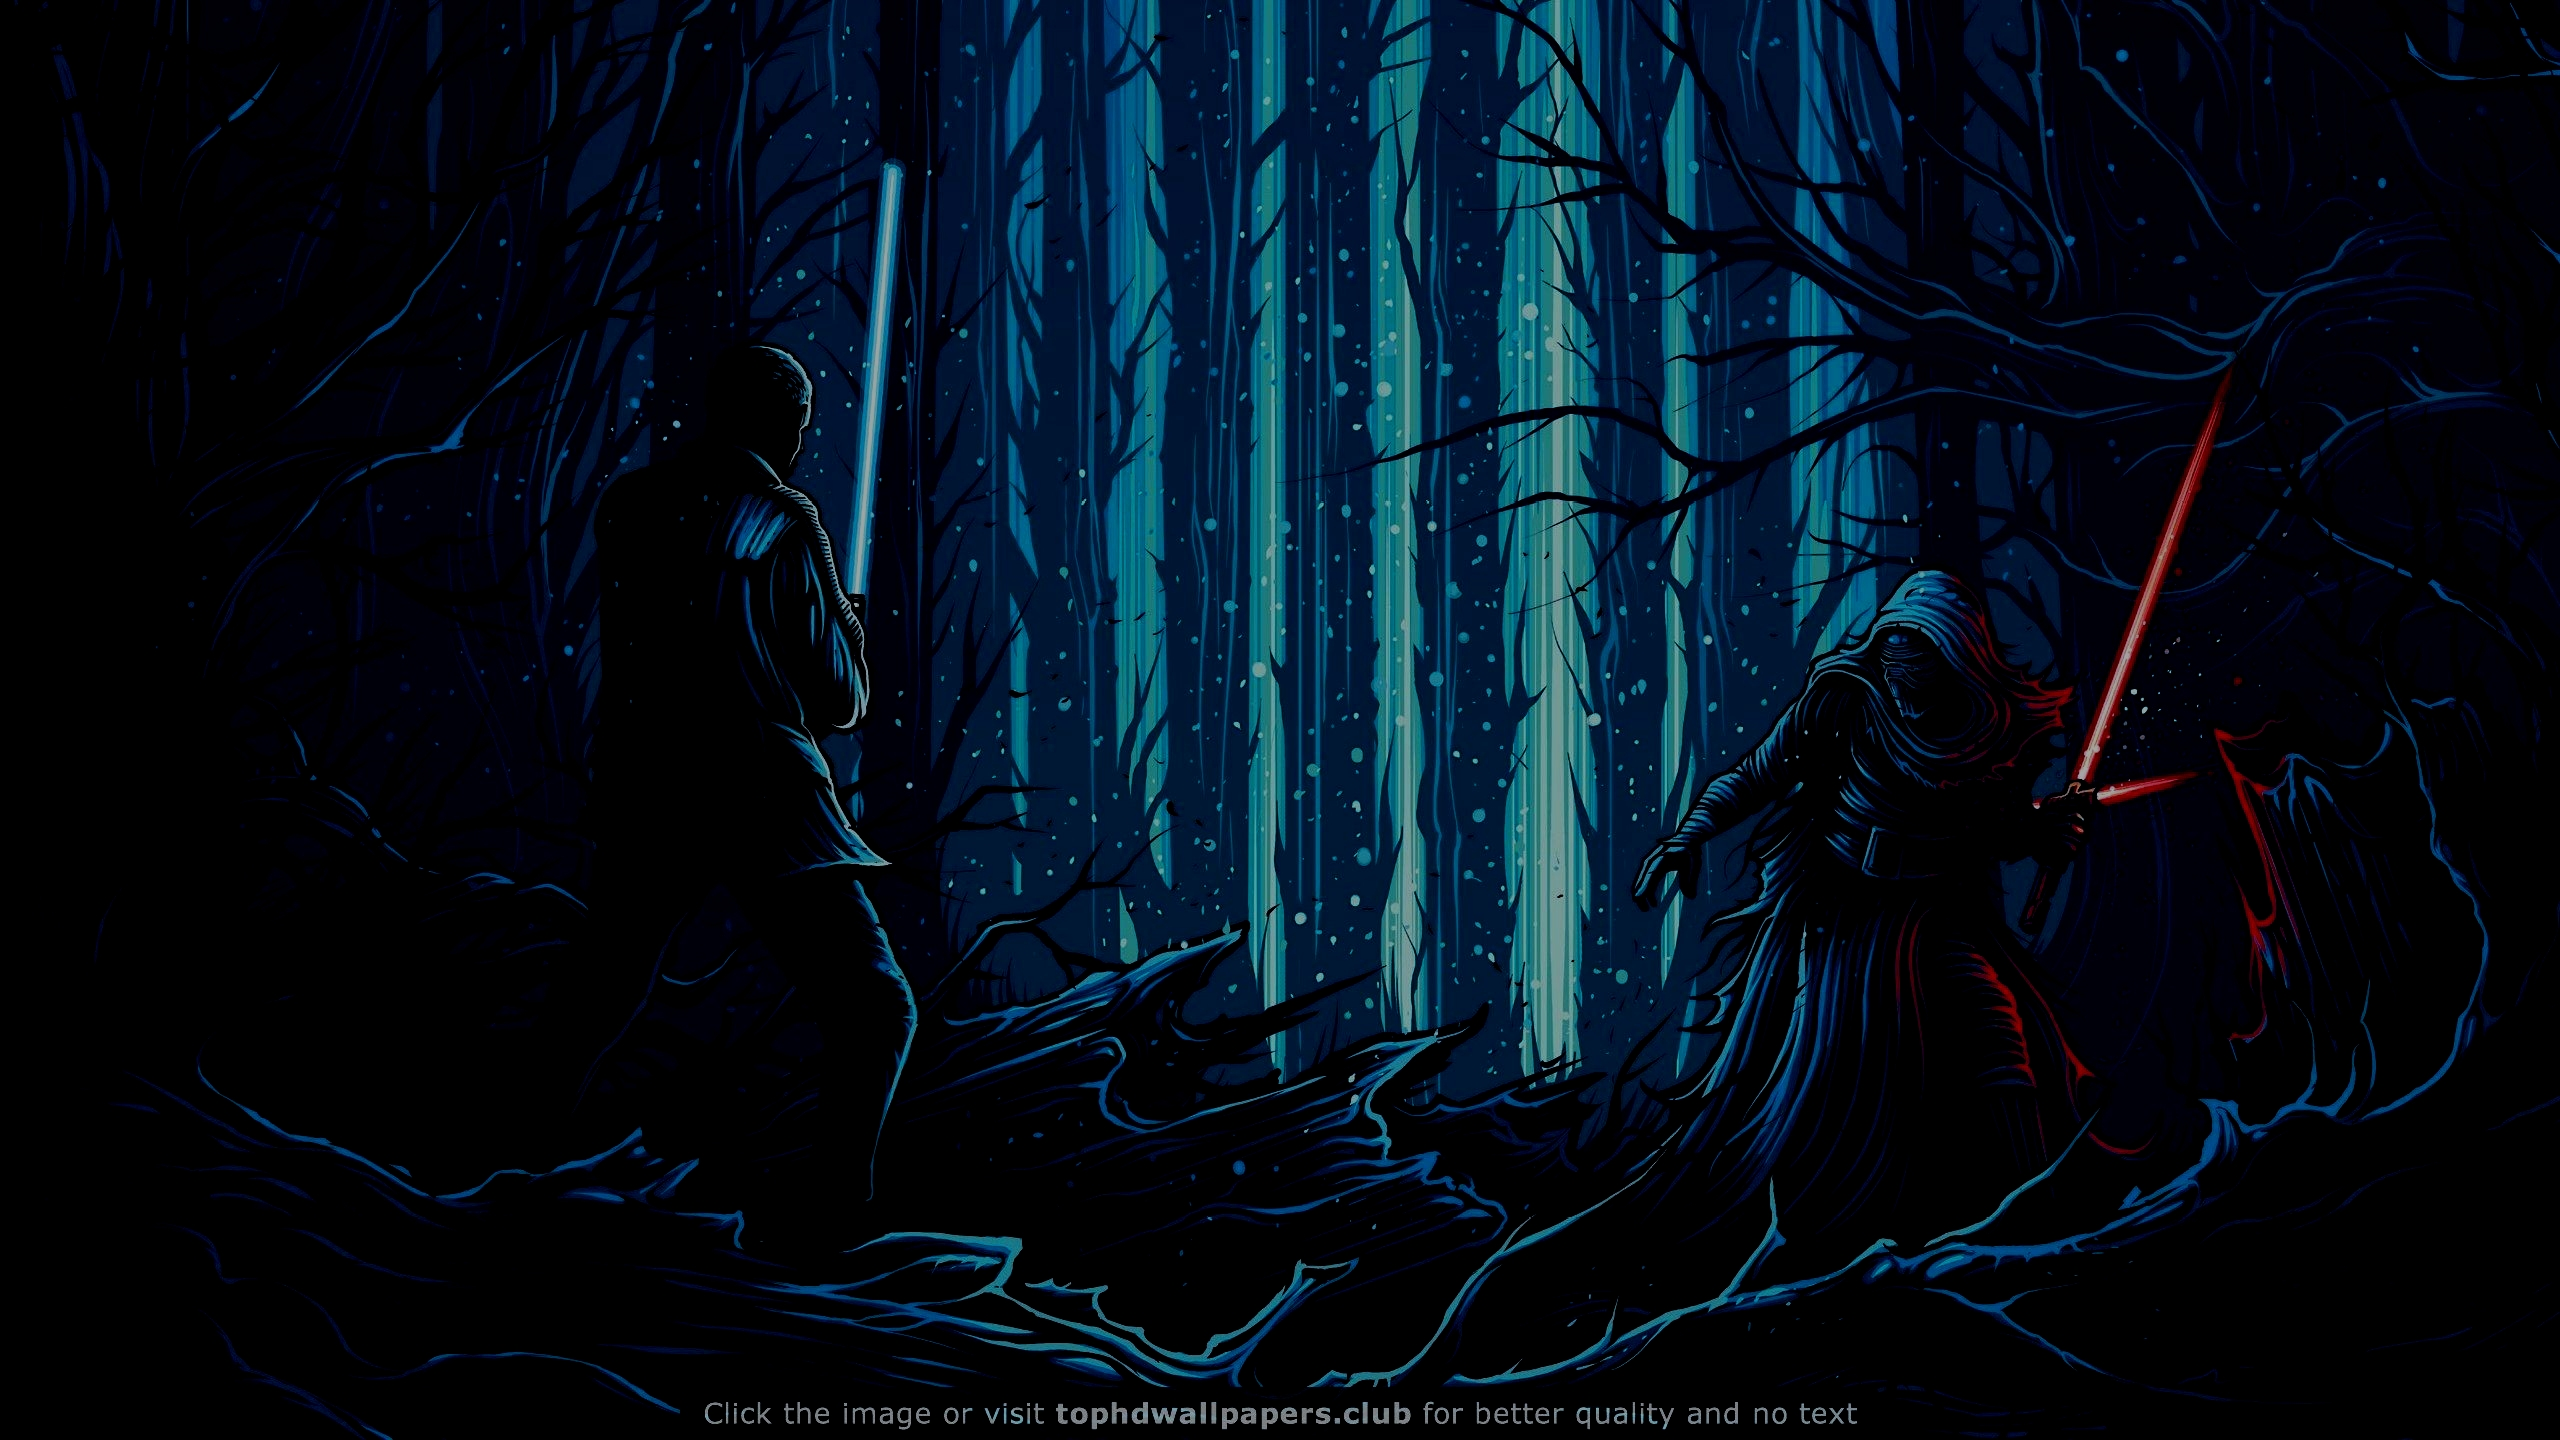
\includegraphics[width=0.5\textwidth]{report_src/brightness_low.jpeg}
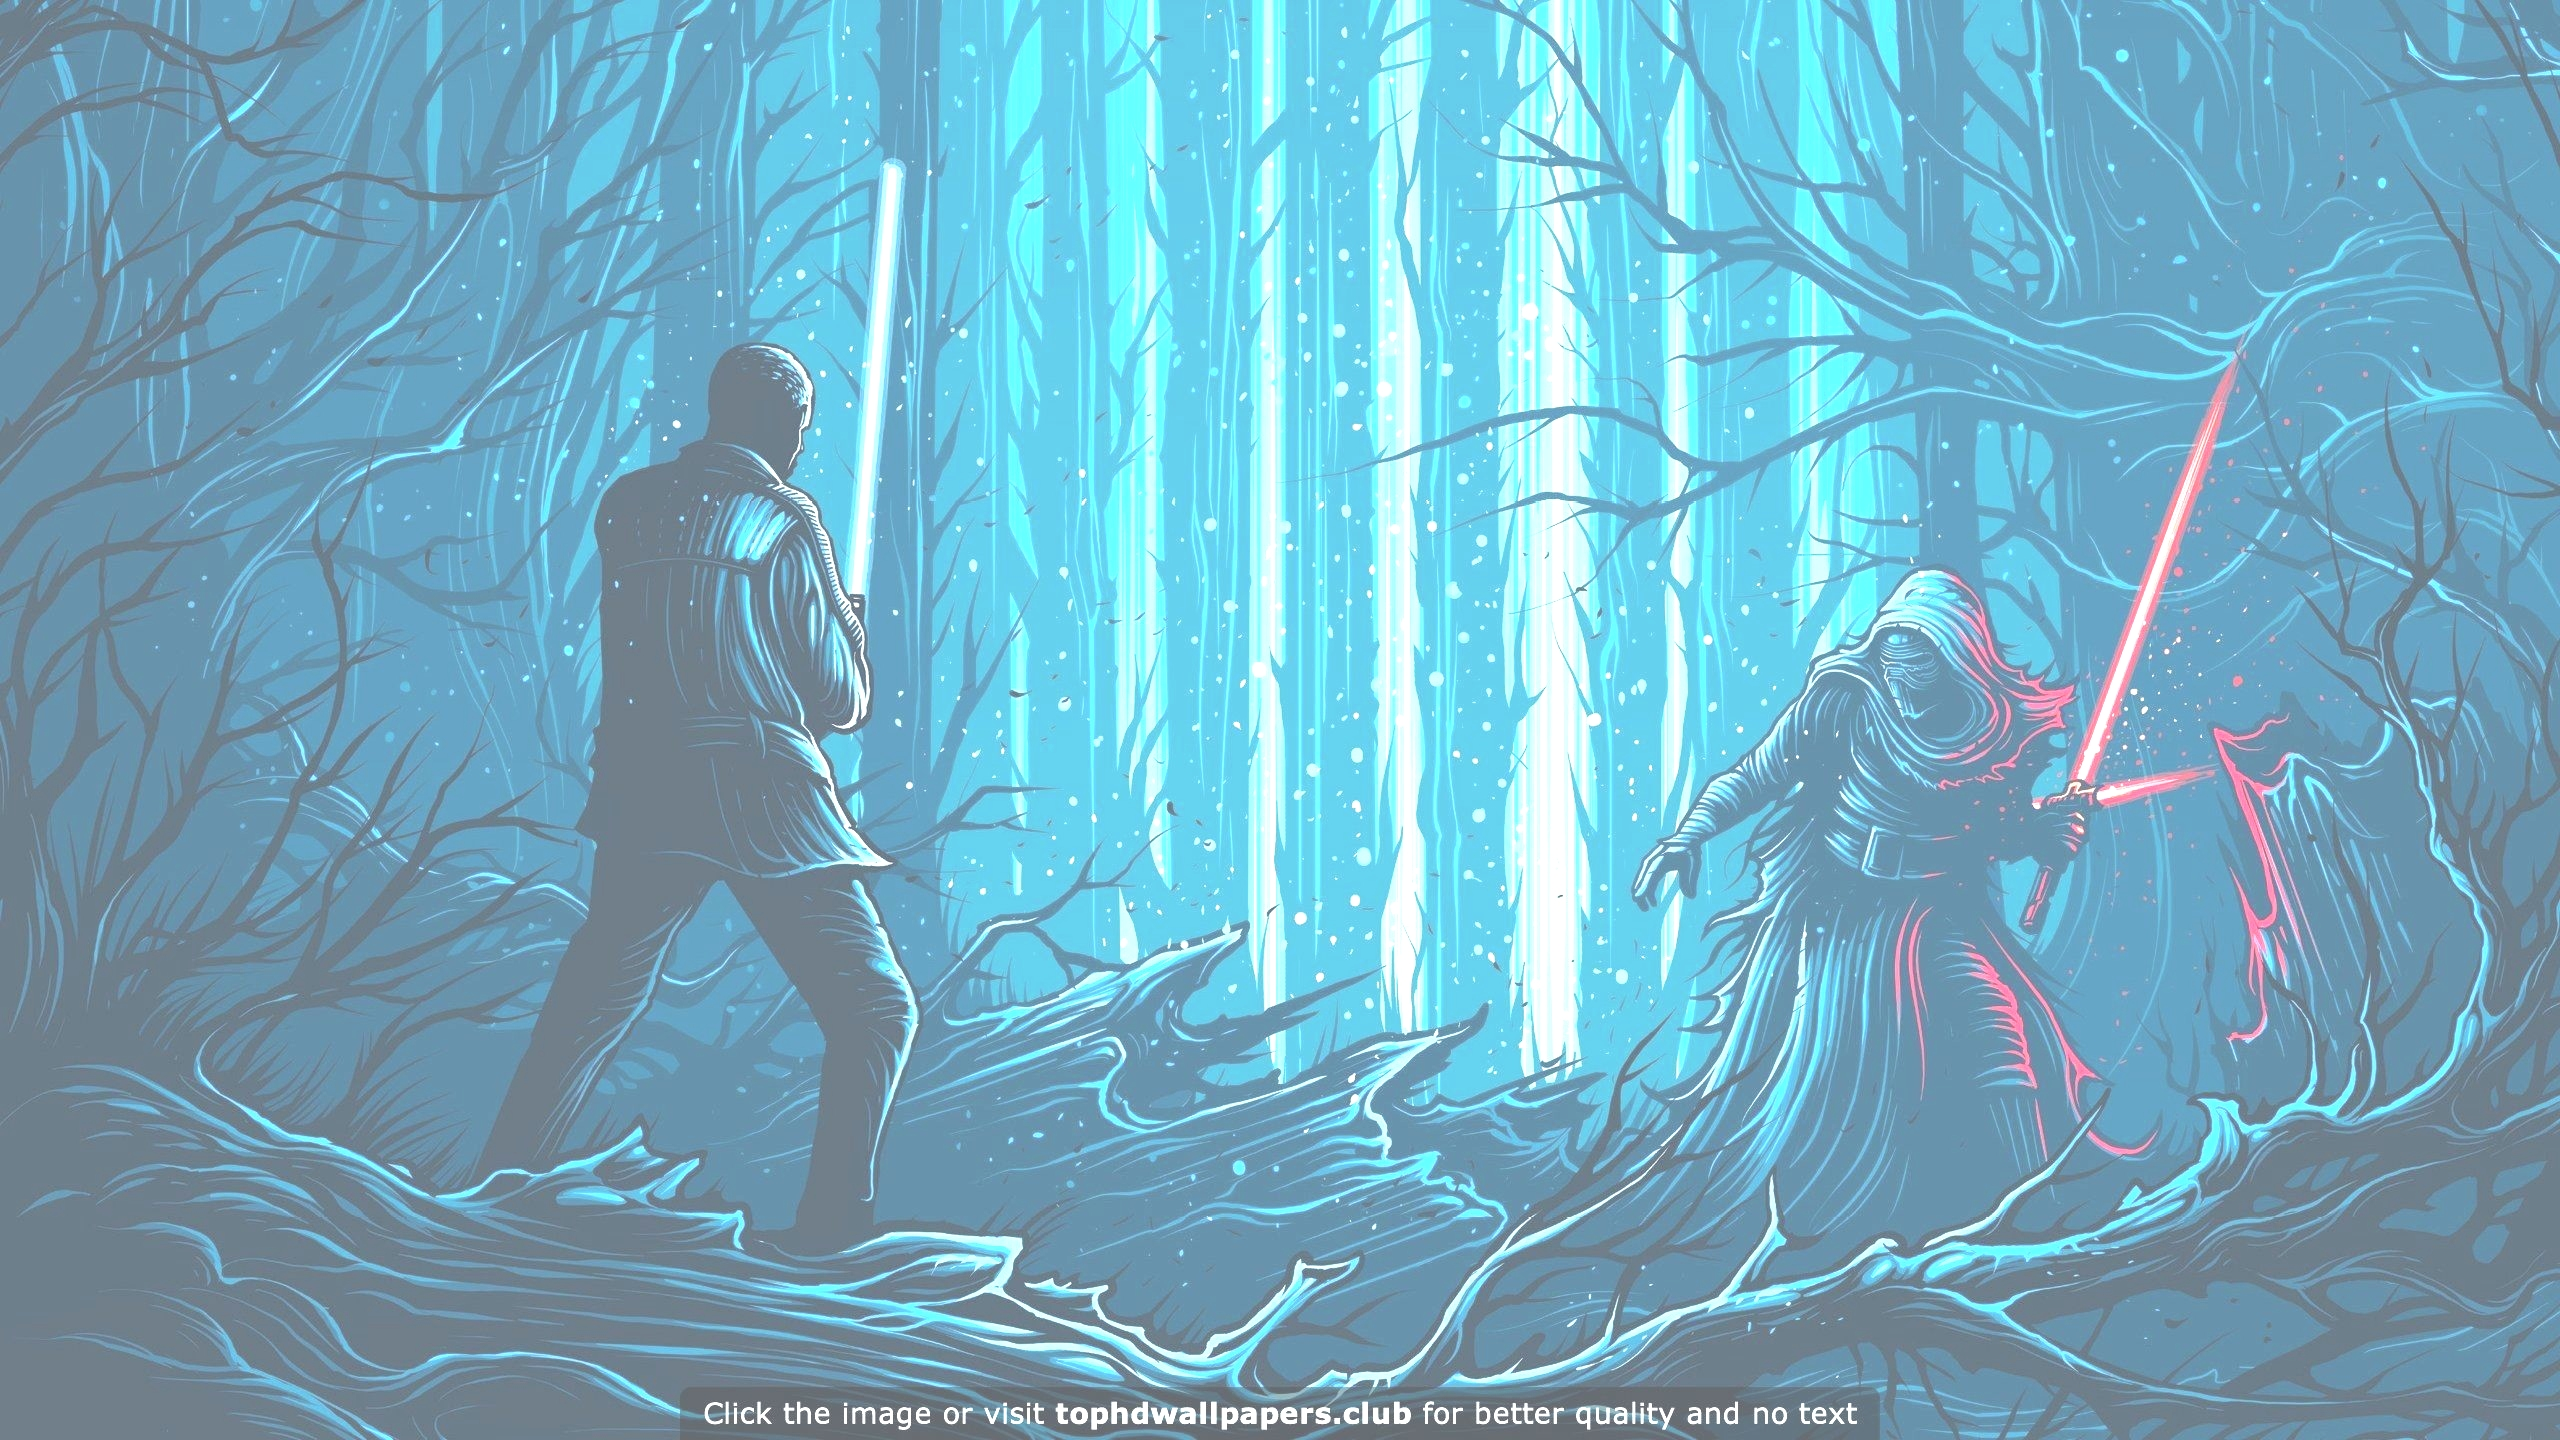
\includegraphics[width=0.5\textwidth]{report_src/brightness_high.jpeg} 

\emph{Méthode appelante : Retouching.setBrightness()}

\emph{Script : brightness.rs}
\\

Ce réglage ajoute une valeur (positive ou négative) aux trois canaux RGB de l'image. Cette valeur est fixée par la seekbar.
Les valeurs sont tronquées entre 0 et 255, par conséquent on perd de l'information dans les valeurs extrêmes de luminosité.

Cet effet n'utilise pas la luminosité existante de l'image, ainsi on peut obtenir des résultats qui sont parfois discutables, par exemple
le noir qui s'éclaircit et inversement pour le blanc. Pour pallier à ce problème, on pourrait introduire une multiplication afin de modifier
la luminosité proportionnellement à celle existante. Cependant, cette solution modifie aussi le contraste, nous avons donc choisi
de laisser l'algorithme tel quel.


\subsection{Contraste (Contrast) :}

\emph{Méthode appelante : Retouching.dynamicExtensionRGB()}

\emph{Script : dynamicExtension.rs}
\\ 

Ce réglage effectue une extension linéaire de dynamique. Les nouveaux extremum de l'histogramme sont définis à partir de la position de la seekbar.
La dynamique est ainsi étendue autour d'une valeur se situant au milieu des deux anciens extremum de l'histogramme*. On a donc une image uniforme lorsque
l'on règle le contraste au minimum. En augmentant le contraste, les extremum peuvent sortir de l'intervalle [0;255], ce qui provoque une distorsion de l'image.
\\

*Il serait peut-être plus judicieux de prendre la médiane de l'histogramme cumulé afin d'avoir une valeur qui représente mieux la "valeur moyenne" de l'image.


\subsection{Saturation (Saturation) :}

\emph{Méthode appelante : Retouching.setSaturation()}

\emph{Script : saturation.rs}
\\

Ce réglage permet de régler la saturation de l'image. Soit S la saturation existante, S' la nouvelle saturation et F le facteur de saturation. S et S' vont de 0 à 1.

On a S' = S + F * (1 - S) * S. 

On observe que la nouvelle saturation est proportionnelle à deux facteurs : l'espace restant avant une saturation totale (1-S) et la saturation existante S.
Par conséquent, en augmentant la saturation, chaque pixel tend vers sa saturation maximale, tout en garantissant une saturation proportionnelle à celle existante, évitant ainsi de saturer le gris.


\subsection{Hue:}

    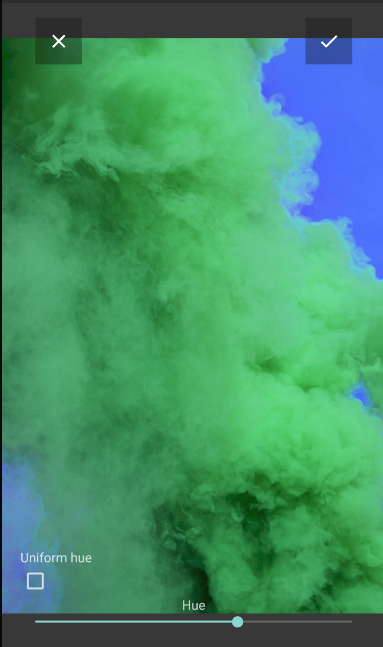
\includegraphics[width=0.25\textwidth]{report_src/non-uniform-hue.png}
    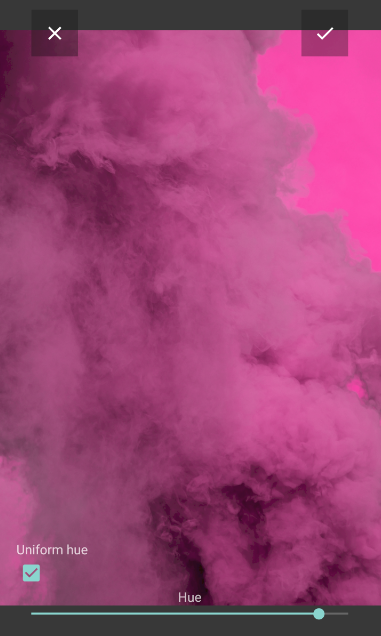
\includegraphics[width=0.25\textwidth]{report_src/uniform-hue.png}
    \newline
    \emph{Méthode appelante : Color.colorize()}

    \emph{Scripts : colorize.rs, utils.rs} 
    \newline
    Ce reglage efectue une conversion des couleurs de chaque pixel du format RGB au HSV puis change le champ Hue du pixel ce qui permet de 
    changer le teint de image.
    Le teint en question est sélectionné par l'utilisateur grâce a la seekbar qui lui est fournie ainsi qu'une option a cocher qui lui propose deux choix:
    \\

    \subsubsection{Teint uniforme:}
        En cochant la case "uniforme" l'effet remplace le teint de tout les pixels de l'image en changeant le champ hue de chaque pixel par celui choisis par l'utilisateur grace à la seekbar.
        

    \subsubsection{Teint non uniforme:}
        En décochant la case "uniforme" ajoute le teint sélectionné par l'utilisateur grace à la seekbar au chanp hue déjà contenu dans chaque pixel donnant un nouveau 
        teint a chaque couleur de l'image.
        


\subsection{Keep hue:}

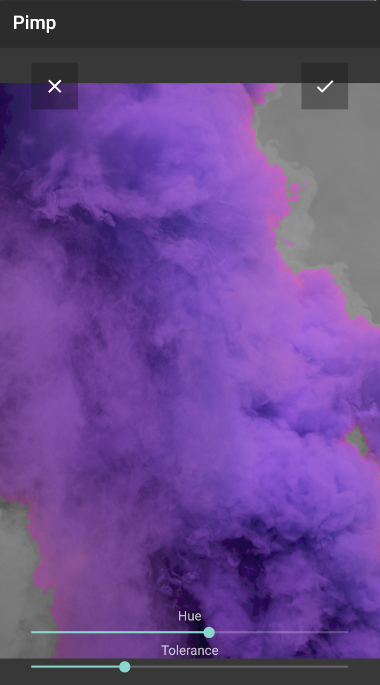
\includegraphics[width=0.25\textwidth]{report_src/keepColor.png}
\newline
\emph{Méthode appelante : Color.keepColor()}

\emph{Scripts : keepColor.rs, utils.rs} 
\newline
Garde qu'un seul teint avec un degré de tolérance sélectionnés par l'utilisateur grâce aux deux seekbars "hue"  et "tolerance" qui lui sont fournies et garde 
le reste des pixels en échelle de gris en convertissant les couleurs de chaque pixel du format RGB au HSV puis gardant que les pixel contenant le hue choisi dans le bon intervalle.
\\




\subsection{Egalisation d'histogramme (Enhance) :}

\emph{Méthode appelante : Retouching.histogramEqualization()}

\emph{Scripts : cumulativeHistogram.rs, assignLut.rs} 
\\

Comme son nom l'indique, cet effet utilise l'égalisation d'histogramme afin d'améliorer le contraste.
On calcule d'abord l'histogramme cumulé et on en déduit la LUT (Look Up Table), que nous assignons ensuite à chaque pixel.
\\

Cependant, afin d'égaliser l'histogramme, l'algorithme éclaircit les zones sombres, ce qui donne un résultat peu convaincant sur les images de faible luminosité.
Une solution à ce problème est l'égalisation d'histogramme adaptative (CLAHE), mais nous n'avons pas eu le temps de l'implémenter pour ce rendu.

\subsection{Convolution (Blur, Sharpen, Neon) :} \label{convolution}

    Dans cette sous-section on retrouve des effets réalisés avec des convolutions pour flouter une image en passant par deux types différents de kernel : Gaussien et moyenneur
    (bouton "Blur"), des effets pour améliorer la netteté d'une image avec la fonction "Laplacian of gaussian" (bouton Sharpen) et des effets de 
    détection de contours (bouton "Neon") en réalisant des convolutions avec des opérateurs comme Sobel, Prewitt, Kirsch ou une convolution simple avec un kernel
    laplacien.
    \\

    Pour ces effets nous avons implémenté 3 méthodes de convolution.


    \begin{itemize}
        \item Convolution classique.
        \item Convolution séparable.
        \item Convolution détection de contours.
    \end{itemize}
    

    \subsubsection*{Convolution classique} \label{conv_classique}
    
        Cette méthode de convolution suit le même algorithme vu en cours, on peut l'appliquer avec des noyaux asymétriques de dimensions impaires uniquement,
        cette opération a été parallélisée grâce à l'outil "renderscript" qui parallélise le calcul par CPU multithreading/GPU. En plus dans cette méthode (et dans toutes les autres) nous avons rajouté
        des optimisations pour parcourir seulement les index nécessaires de l'image lors de la convolution. En calculant les index des centres des deux dimensions du kernel
        on peut anticiper et éviter les appels de fonction inutiles sur les bords de l'image par exemple.
        
        $X_{d\acute{e}but}$ et $X{fin}$ étant le premier et dernier index à parcourir dans l'axe des abscisses respectivement et
        $Y_{d\acute{e}but}$ et $Y_{fin}$ étant le premier et dernier index à parcourir dans l'axe des ordonnées respectivement.
        \[
            Kernel_{CentreX} =   \frac{Largeur_{kernel}}{2}            
        \]
        \[
            Kernel_{CentreY} =   \frac{Hauteur_{kernel}}{2}            
        \]
        \[
            X_{d\acute{e}but} = Kernel_{CentreX}      
        \]
        \[
            X_{fin} = Largeur_{image} - Kernel_{CentreX}           
        \]
        \[
            Y_{d\acute{e}but} = Kernel_{CentreY}      
        \]
        \[
            Y_{fin} = Hauteur_{image} - Kernel_{CentreY}           
        \]

        En définissant les index du début et de fin de parcours pour les deux dimensions de l'image sur le script de lancement renderscript
        comme ci-dessus on peut s'en passer de quelques appels de fonctions sur les bords de l'image et ainsi gagner du temps de calcul.

    \subsubsection*{Convolution séparable} \label{conv_separable}

        Pour la convolution classique avec un kernel de taille $N*M$ on doit faire $N*M$ multiplications pour chaque échantillon,
        cependant si le kernel est séparable on peut passer à $N+M$ opérations. Voir \ref{separable_source}.
        \\

        Or afin d'optimiser le calcul de la convolution sur des filtres séparables comme le filtre gaussien et moyenneur nous avons implémenté une
        méthode de convolution séparable.
        
        \begin{figure}[!h]
            \centering
            \begin{subfigure}[b]{1\textwidth}
                \centering
                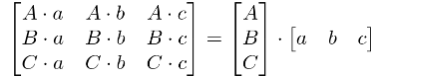
\includegraphics[width=0.5\textwidth]{report_src/separableConv1.png}
            \end{subfigure}
        \end{figure}

        Un kernel est séparable quand sa matrice des poids peut être représentée par le produit de deux vecteurs.
        \\

        Ce calcul est réalisé en faisant deux convolutions unidimensionnelles successives (en X et en Y) sur l'image d'origine en stockant le résultat dans une image intermédiaire.
        La propriété d'associativité de la convolution rend ce calcul possible.

        \[
            x * (N * N)  \iff (x * N) * N
        \]

        La limite de cette méthode c'est que l'on doit passer par une image partielle pour la réalisation du calcul en
        utilisant plus de mémoire que pour une convolution classique.
        \\



    \subsubsection*{Convolution détection de contours} \label{conv_edges}

        Cette méthode prend en paramètre deux kernels de même taille et réalise deux convolutions avec chaque kernel et ensuite calcule le produit des deux.
        Vu que ces deux convolutions sont indépendantes l'une de l'autre on peut se permettre de les réaliser au même temps dans le script et de faire l'addition
        des valeurs absolues résultantes des deux accumulateurs. Comme son nom l'indique cette méthode est utilisée notamment pour faire des convolutions pour la détection de contours
        avec des opérateurs comme Sobel, Kirsch, Prewitt, etc.
    \\
        

    \subsubsection*{Padding} \label{padding}

        Pour éviter l'effet conséquent de la convolution qui est la perte de bords, on applique un padding par extension depuis renderscript.
        \begin{figure}[!h]
            \centering
            \begin{subfigure}[b]{0.3\textwidth}
                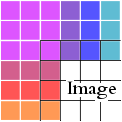
\includegraphics[width=1\textwidth]{report_src/effects/padding.png}
            \end{subfigure}
            \caption*{Exemple de padding par extension.}
        \end{figure} 


    \subsubsection*{Les kernels} \label{kernels}

        Tous les kernels sont définis dans la classe fr.ubordeaux.pimp.util.Kernels. Les kernels de détection de contour (Sobel, Kirsch, Laplace, Prewitt) sont définis
        en variable statique et finale, car leur taille est fixe, les autres sont générés par une méthode. Si on prend le cas du kernel de Gauss, la méthode gauss permet 
        de générer la version séparée du kernel, c'est-à-dire une seule ligne. Les méthodes génératrices de kernel prennent en argument la taille de celui-ci, ce qui sert
        aux effets paramétrables tels que blur et sharpen.

    \subsubsection{Flou gaussien et moyenneur (Blur) : } \label{blur}

        \begin{figure}[!h]
            \centering
            \begin{subfigure}[b]{0.3\textwidth}
                \includegraphics[width=1\textwidth]{report_src/effects/original.jpeg}
            \end{subfigure}
            \begin{subfigure}[b]{0.3\textwidth}
                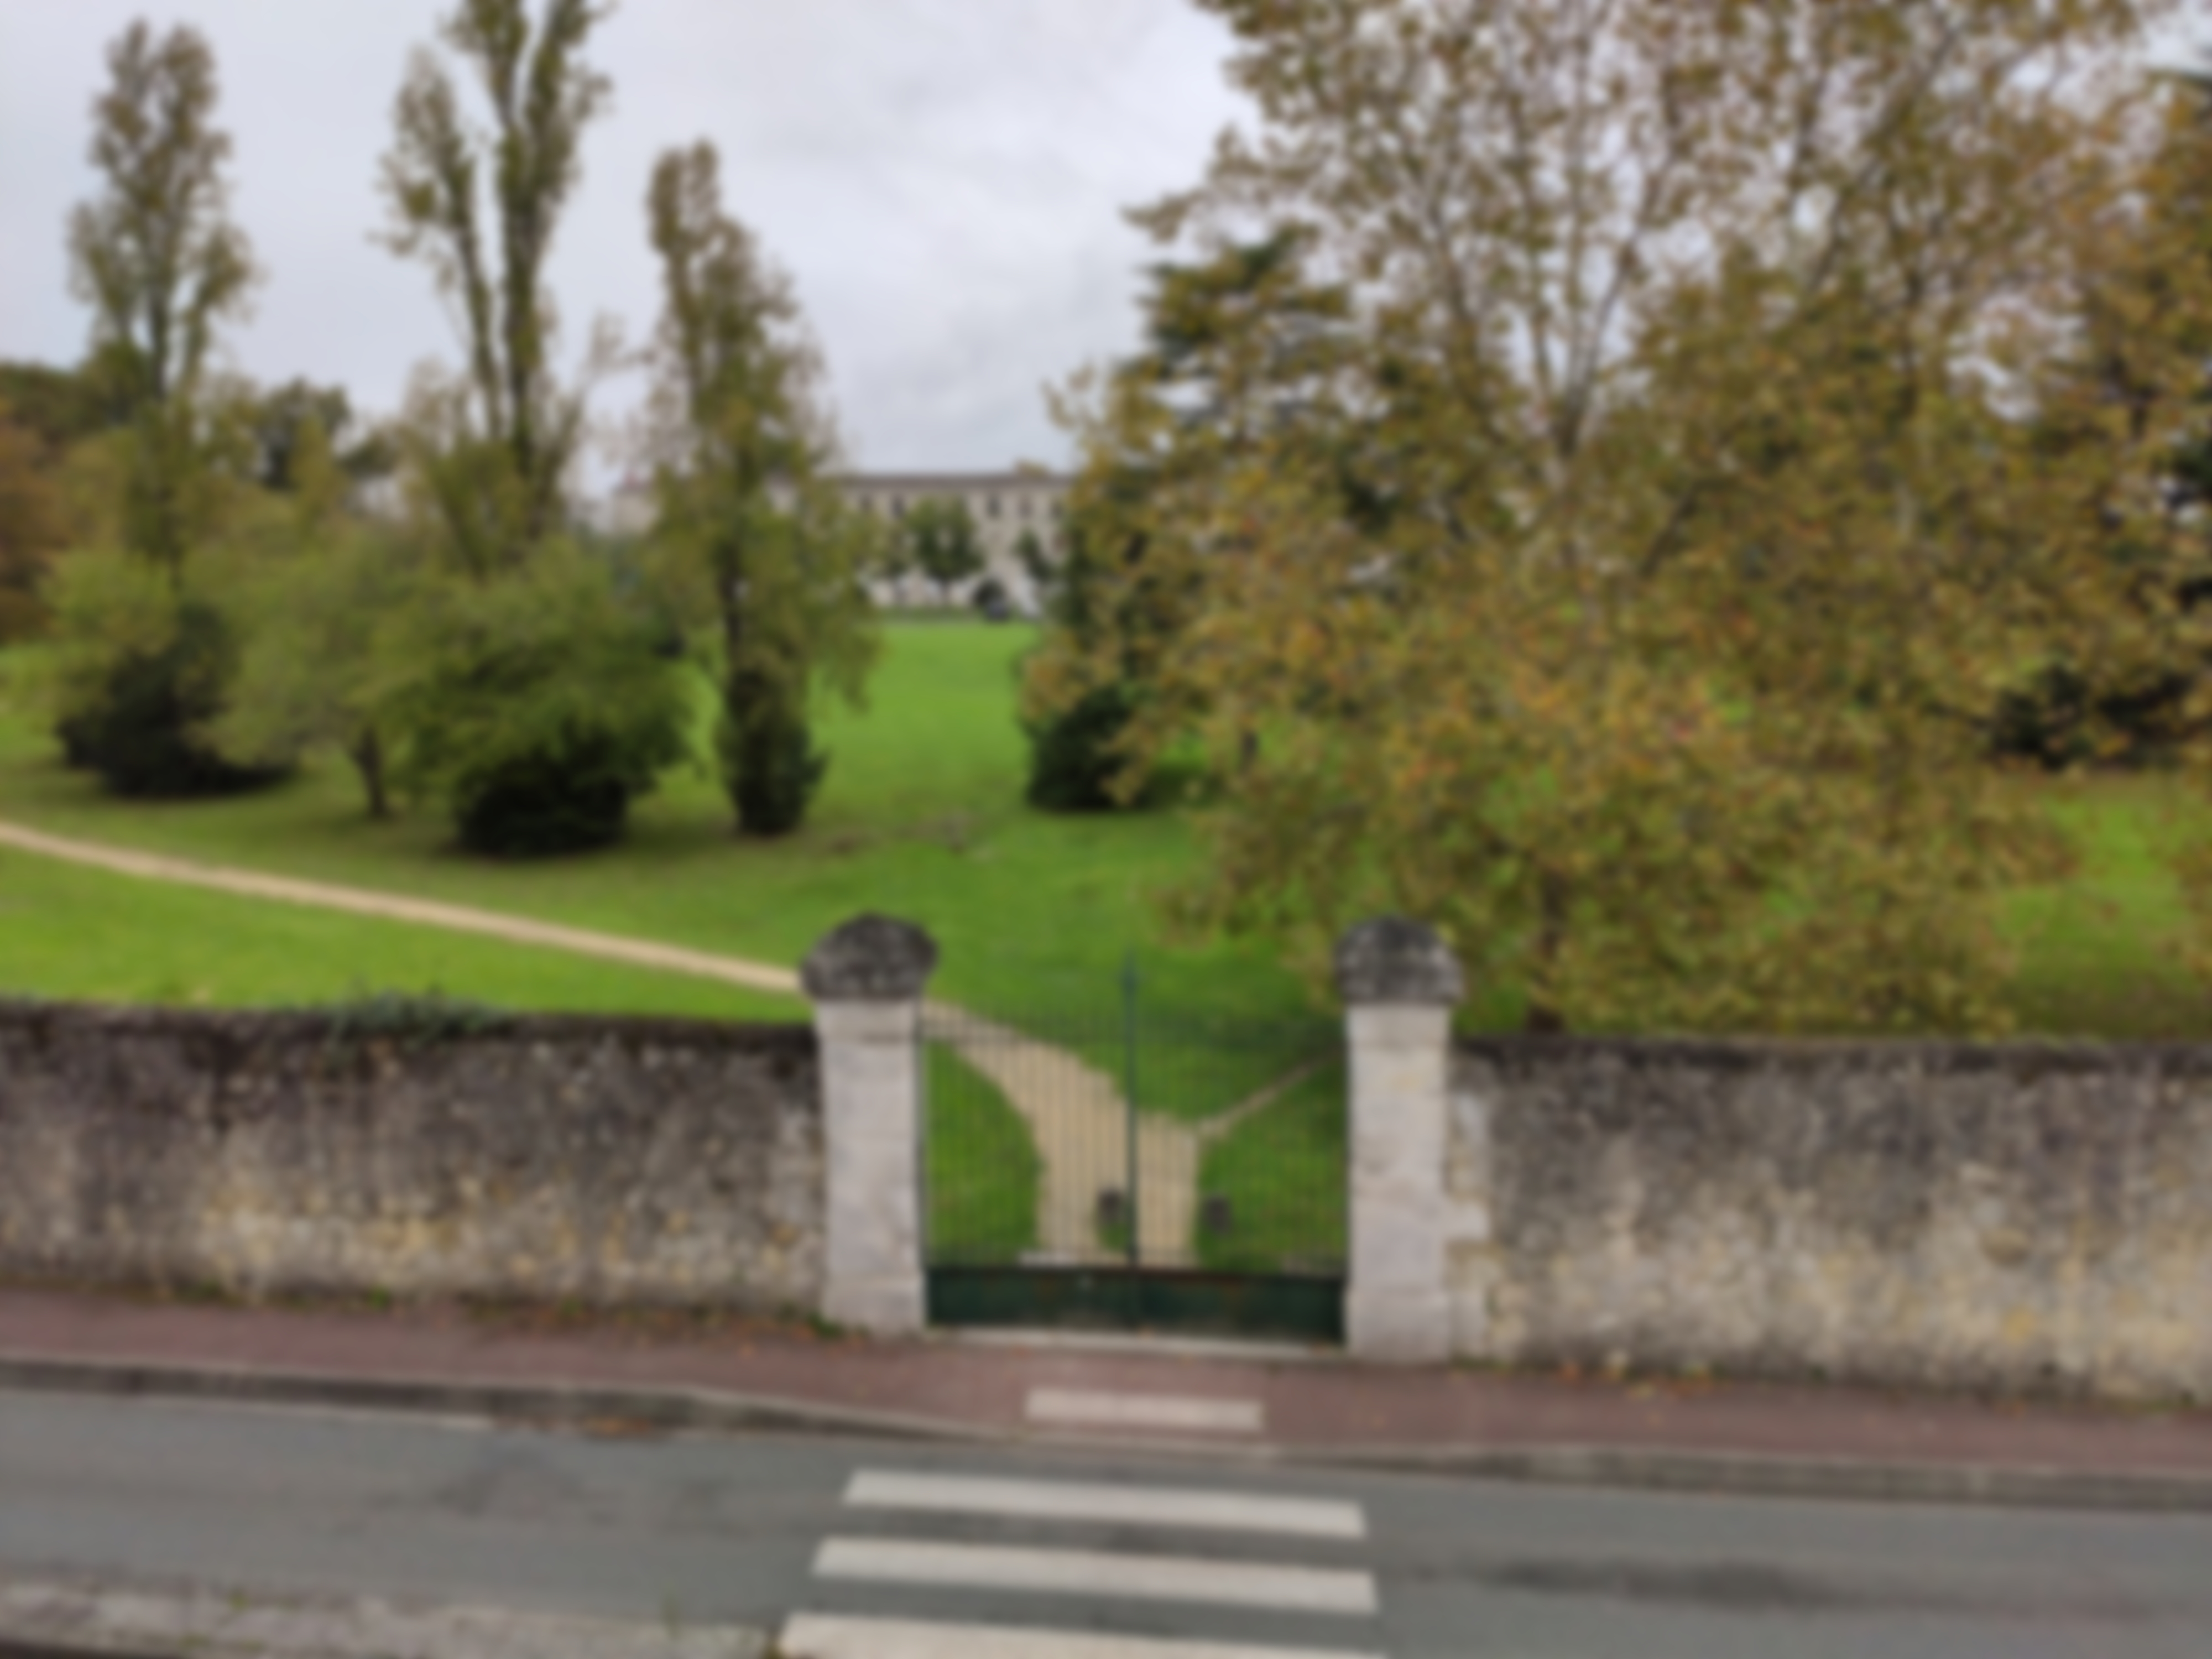
\includegraphics[width=1\textwidth]{report_src/effects/blur.jpeg}
            \end{subfigure}
            \begin{subfigure}[b]{0.3\textwidth}
                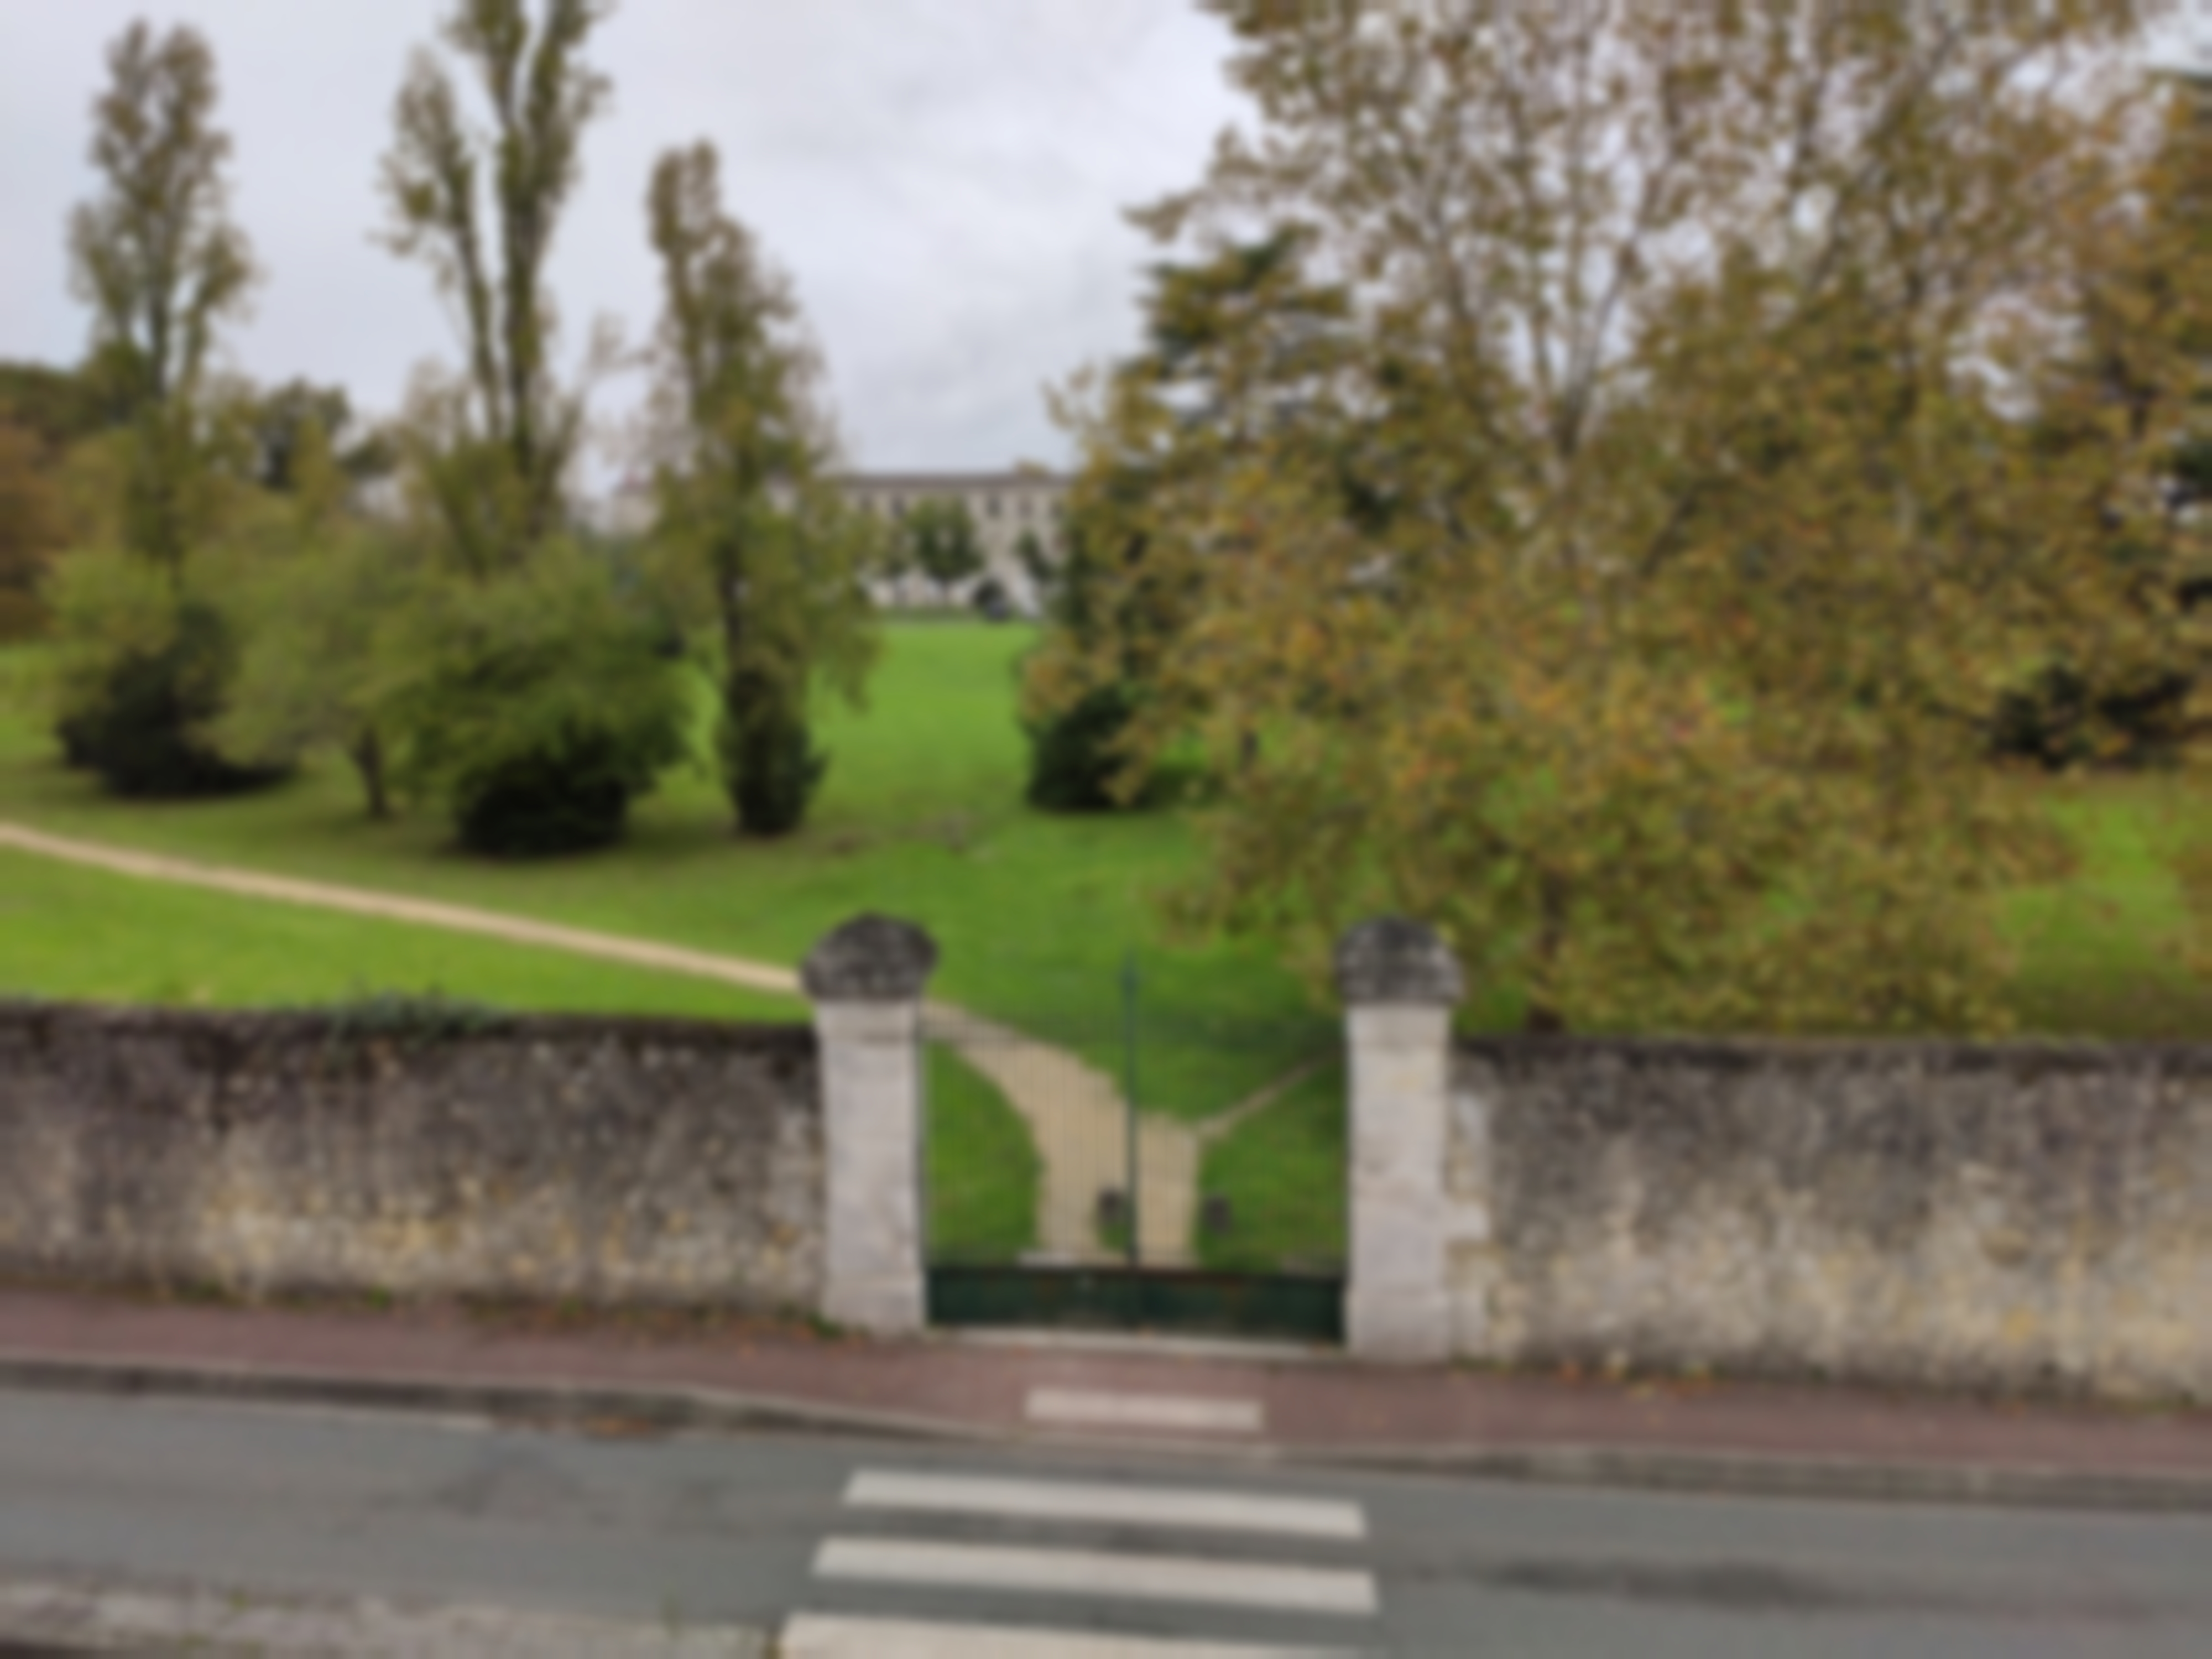
\includegraphics[width=1\textwidth]{report_src/effects/mean.jpeg}
            \end{subfigure}
            \caption*{Comparaison des deux filtres Gaussien(2ème image) et Moyenneur(3ème image) sur une image de taille 4000x3000px.}
        \end{figure} 
        \emph{Méthodes appelantes : Convolution.gaussianBlur(), Convolution.meanBlur()}

        \emph{Scripts : convolution.rs} 

        Dans la section blur, on réalise des convolutions avec un filtre gaussien ou moyenneur selon le choix de l'utilisateur,
        ces filtres sont réalisés avec une méthode de convolution séparable voir \ref{conv_separable}. Ces kernels sont générés en fonction du progrès de la seekbar qui
        définit une taille de vecteurs allant de l'intervalle [3 - 25]. Pour le filtre gaussien l'écart type noté $\sigma$ est généré en fonction de la taille du kernel en suivant
        cette relation.
        \[
            \sigma  =  \frac{taille_{kernel}}{2}            
        \]

        Cette relation a été définie arbitrairement car il y n'y a pas moyen de calculer avec certitude l'écart type de la fonction gaussienne et en fonction des résultats
        obtenus après une série des tests on a décidé de laisser la relation de ci-dessus.

        Pour le filtre moyenneur tout comme le filtre gaussien on génère un vecteur de taille dans l'intervalle [3 - 25] et on les applique verticalement et ensuite horizontalement
        avec la méthode de convolution séparable.
        \\
        
        Cet effet s'applique en temps réel sur l'image et pourtant doit être assez rapide pour son utilisation, il restent encore quelques optimisations à faire
        pour améliorer la fluidité de ce dernier. Voir \ref{limits_conv}.
        \\
        \newpage


    \subsubsection{Amélioration de la netteté / Masque flou (Sharpen) : } \label{sharpen}

        \begin{figure}[!h]
            \centering
            \begin{subfigure}[b]{0.4\textwidth}
                \includegraphics[width=1\textwidth]{report_src/effects/original.jpeg}
            \end{subfigure}
            \begin{subfigure}[b]{0.4\textwidth}
                \includegraphics[width=1\textwidth]{report_src/effects/sharpen.jpeg}
            \end{subfigure}
            \caption*{Application de filtre LoG, kernel de taille 13x13, $\sigma$ = 2.6 et image de 4000x3000px}
        \end{figure} 
        
        \begin{figure}[!h]
            \centering
            \begin{subfigure}[b]{0.4\textwidth}
                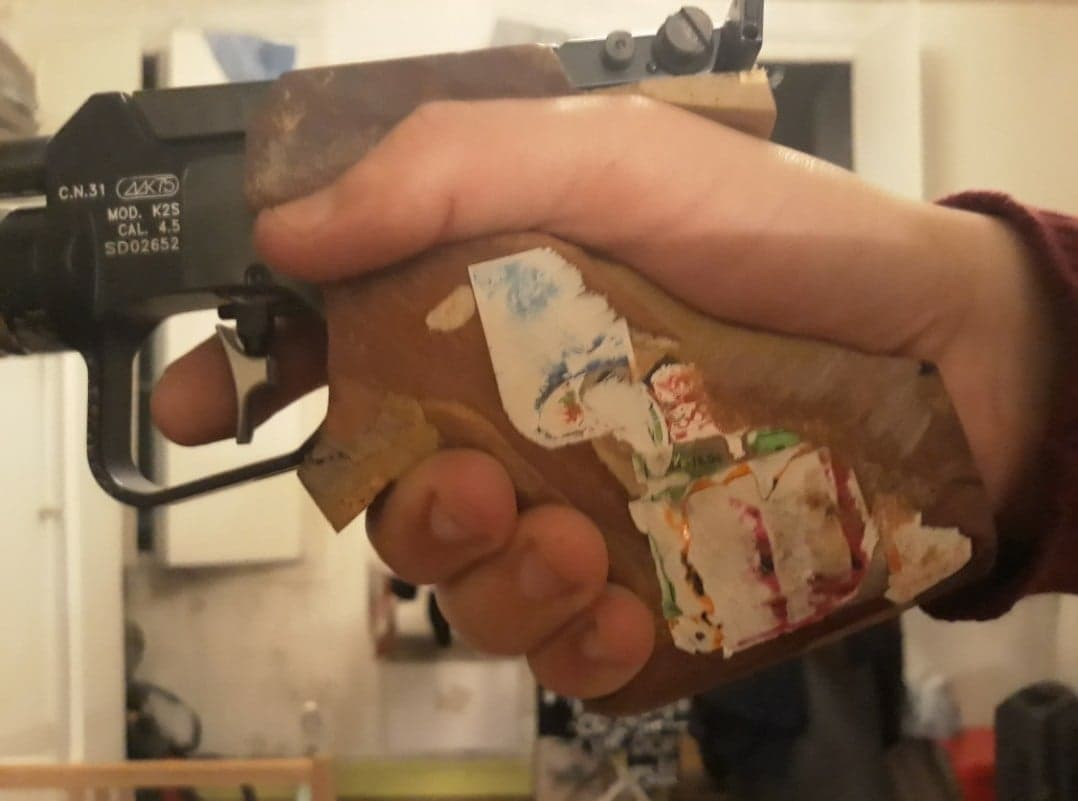
\includegraphics[width=1\textwidth]{report_src/effects/sharpen2.jpg}
            \end{subfigure}
            \begin{subfigure}[b]{0.4\textwidth}
                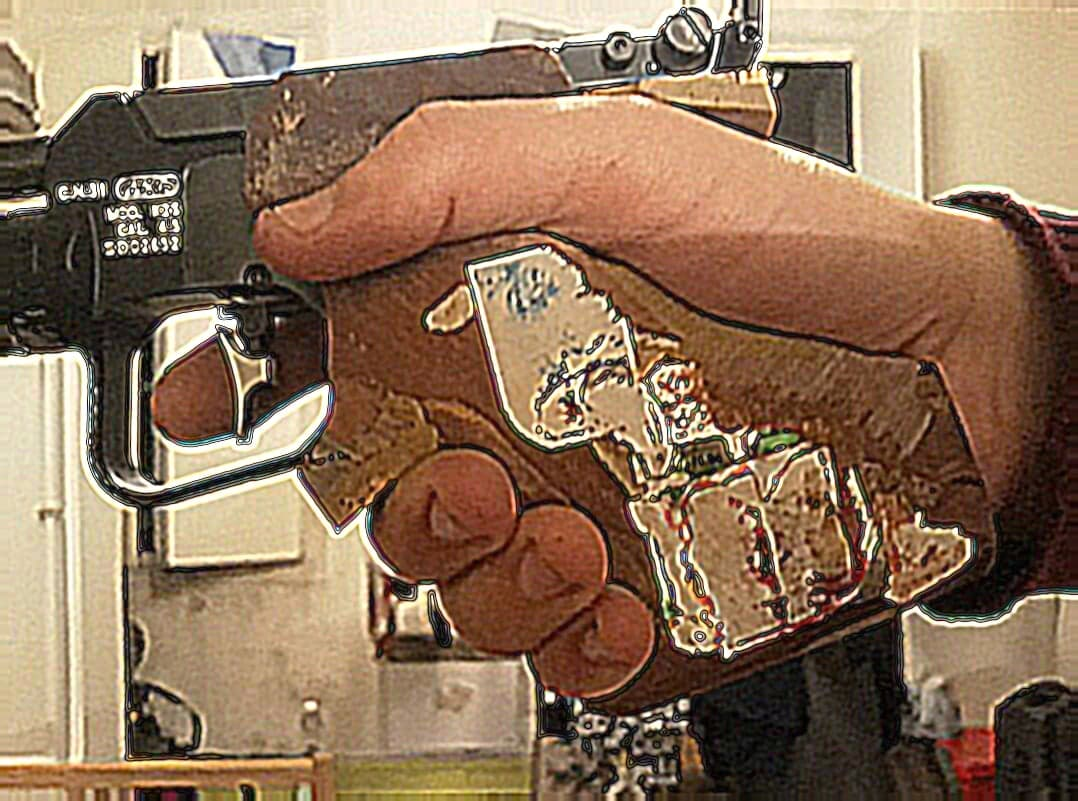
\includegraphics[width=1\textwidth]{report_src/effects/org2.jpg}
            \end{subfigure}
            \caption*{Application de filtre LoG, kernel de taille 9x9, $\sigma$ = 1.8 et image de 1024x724px}
        \end{figure} 
 


        \emph{Méthode appelante : Convolution.sharpen()}
        \emph{Scripts : convolution.rs} 
        \\

        Cet effet consiste à rehausser les contours dans une image également que d'enlever le possible flou dans une image, avec une seekbar en progression.
        Le filtre est réalisé par la convolution d'un filtre suivant une distribution discrète de la fonction "Laplace of Gaussian" (LoG) voir \ref{LoG},
        ce filtre est pourtant séparable en 4 convolutions mais pour histoire d'implémentation et de temps on s'est contenté de garder la version avec la convolution classique.
        Ce filtre est réalisé en temps réel avec des kernels de taille en allant de taille 3x3 jusqu'à 13x13.

        
        \begin{figure}[!h]
            \centering
            \begin{subfigure}[b]{0.8\textwidth}
                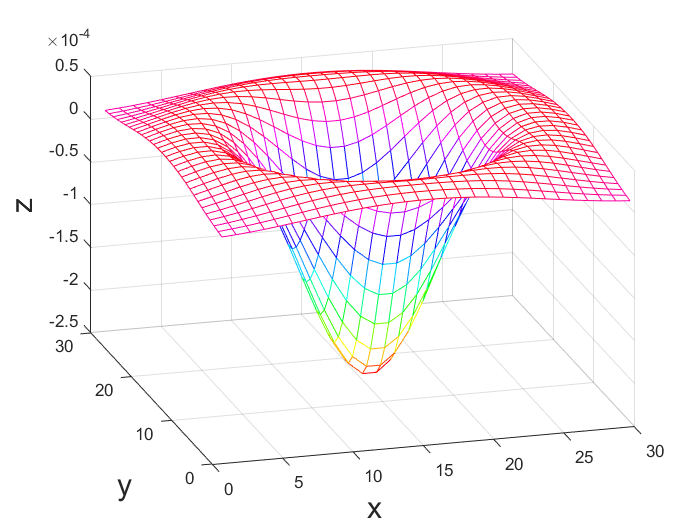
\includegraphics[width=1\textwidth]{report_src/effects/laplacianGaussian.png}
            \end{subfigure}
            \caption*{Représentation graphique de LoG}
        \end{figure}

        Le filtre Laplacien étant très sensible au bruit, c'est pour ceci que généralement on applique une convolution avec un filtre gaussien avant pour supprimer ce bruit,
        cependant avec LoG on peut appliquer une distribution Gaussienne au filtre Laplacien afin d'éviter de faire 2 convolutions.
        \\
        Par ailleurs pour reproduire cet effet de rehaussement de contours on peut
        flouter l'image originale avec un filtre gaussien (suppression du bruit), ensuite calculer la charte de contours avec un filtre laplacien et puis combiner l'image d'origine avec le résultat
        de la charte de contours.
        Grâce à cette fonction on peut compresser cette procédure à une génération de kernel suivi d'une seule convolution de ce dernier.
        \\

        Comme pour les filtres précédents l'écart type du LoG est définit comme suit :
        \[            
            \sigma =  \frac{taille_{kernel}}{5}
        \]

        Comme pour l'écart type gaussien ce sigma a été choisi en fonction des résultats.
        \newpage

    \subsubsection{Détection des contours (Néon) : } \label{neon}

        \begin{figure}[!h]
            \centering
            \begin{subfigure}[b]{0.4\textwidth}
                \includegraphics[width=1\textwidth]{report_src/effects/original.jpeg}
            \end{subfigure}
            \begin{subfigure}[b]{0.4\textwidth}
                \includegraphics[width=1\textwidth]{report_src/effects/sobel.jpeg}
            \end{subfigure}
            \caption*{Opérateur de Sobel sur une image de taille 4000x3000px}
        \end{figure} 
        
        \begin{figure}[!h]
            \centering
            \begin{subfigure}[b]{0.4\textwidth}
                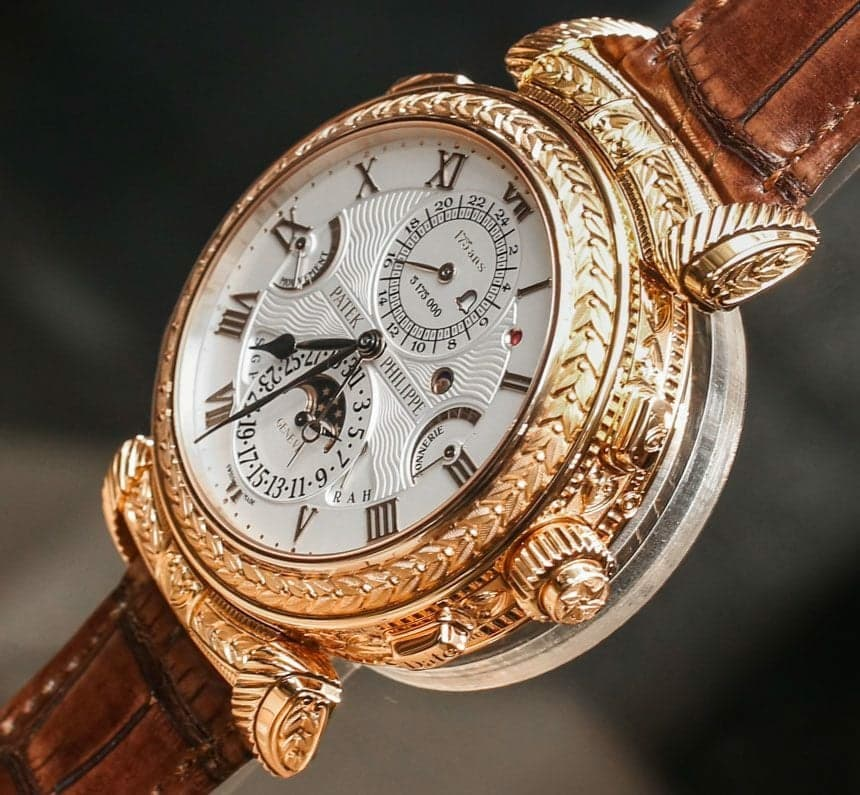
\includegraphics[width=1\textwidth]{report_src/effects/org3.jpg}
            \end{subfigure}
            \begin{subfigure}[b]{0.4\textwidth}
                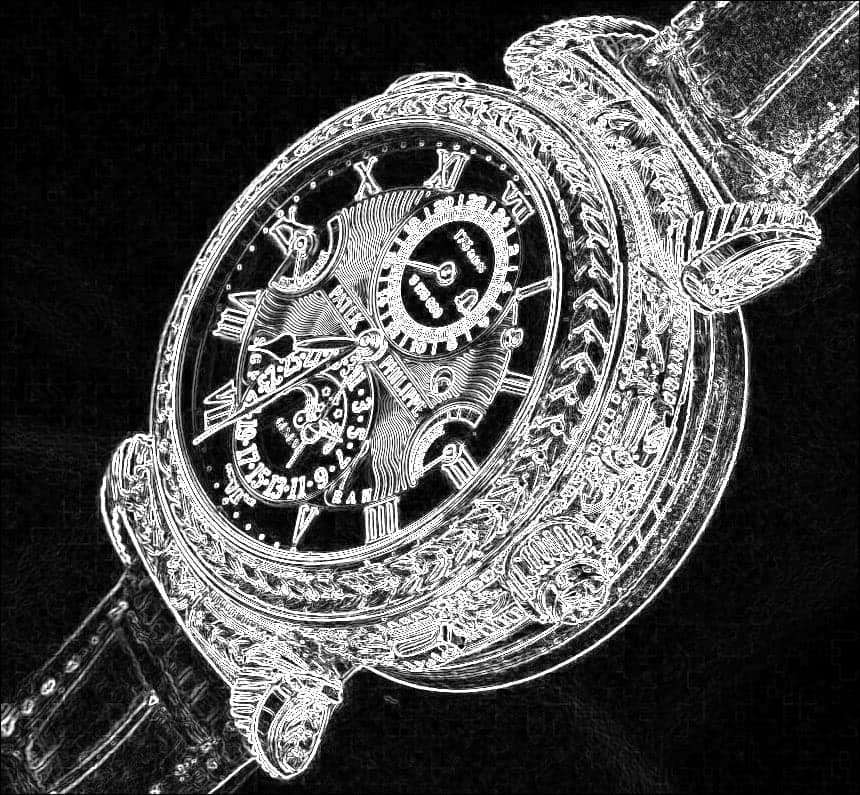
\includegraphics[width=1\textwidth]{report_src/effects/sobel3.jpg}
            \end{subfigure}
            \caption*{Opérateur de Sobel sur une image (passée en échelle de gris) de taille 860x795}
        \end{figure} 

        \emph{Méthode appelante : Convolution.neonSobel()}

        \emph{Scripts : convolution.rs} 
        \\

        Cet effet consiste à créer un effet "Neon" sur une image en utilisant des opérateurs de détection de contours (voir \ref{edge_source}) comme Sobel, Prewitt et aussi d'un filtre Laplacien qui est également détecteur de contours.
        On a mis 3 boutons de type \textbf{RadioButton} pour sélectionner le type de kernel à utiliser et ainsi voir les différences de chacun sur l'image.
        \\
        
        Les valeurs résultantes de la convolution en "Neon" ne sont pas normalisées par extension linéaire, elles sont justes tronquées entre [0 - 255], pour avoir un résultat plus fidèle, faudrait passer par une image intermédiaire, calculer 
        leur respective minimum et maximum pour ensuite normaliser l'image précédente cette solution est discutable puisque on devrait réallouer une image de plus en mémoire. Cependant
        nous avons essayé de \textbf{calculer la valeur maximale théorique} pour normaliser mais ceci donne des résultats très sombres par rapport à l'image originale, nous avons décidé donc de garder l'ancienne normalisation et considérer le fait de normaliser par extension linéaire.
        \\

    \subsubsection{Remarques et limites} \label{limits_conv}

        
        \begin{itemize}
            \item {Un des points de réflexion sur la convolution c'est que jusqu'à présent elle est réalisée sur les 3 canaux RGB, ce qui est assez lourd au niveau de calcul,
            cependant on pourrait passer l'image en échelle de gris et la faire seulement sur un des canaux ou passer pour l'espace HSV en utilisant la value ou la saturation.}
            \item {Tous les calculs de convolution sont uniquement réalisées avec des nombres "flottants", ceci est un choix d'implémentation car renderscript, possède plus de support
            pour réaliser des opérations flottantes que pour des opérations sur des entiers qui en plus sont codés en 8 bits dans une image. Pour éviter donc les erreurs de débordement et pour garder une bonne qualité de l'image
            on a décidé de travailler exclusivement avec des flottants, même si ceci peut être pénalisant au niveau de performance, cependant des tests sont à prévoir pour le prochain rendu pour essayer
            d'améliorer la performance sur des filtres comme "Blur"\ref{blur} et "Sharpen"\ref{sharpen}.}
            \item {Pour la convolution classique et séparable les valeurs sont normalisées en divisant le résultat d'opération de voisinage pour un pixel donné
            divisé par la somme des poids des éléments du kernel. Ceci marche assez bien sauf pour les kernels avec des valeurs négatives notamment ceux de détection de contours comme Laplace, Sobel, Prewitt, etc (Voir \ref{conv_edges}).
            }

            \item {Il y a quelques améliorations de performances à faire pour les convolutions réalisées en temps réel comme pour les effets Blur et Sharpen, une optimisation par échantillonnage linéaire\ref{linear_sampling}
            est à tester ainsi que le calcul par des entiers au lieu de flottants.}

            \item {Une des plus grandes limites des effets de convolution c'est que dû à notre implémentation de sauvegarde\ref{file_effets}, on ne peut malheureusement pas garantir le même résultat sur l'image sauvegardée que sur l'aperçu.
            Vu que la réponse des filtres de convolution sur une image précise sont fortement liés à la taille de l’image et que l'image d'aperçu est en général plus petite que l'originale, de fois on peut se retrouver avec une image sauvegardée avec un flou moins fort ou avec une détection de bords plus faible que sur l'aperçu
            ainsi qu'une sensibilité plus forte au bruit.\ref{remarques_code}}
        \end{itemize} 





        
